\documentclass[12pt,a4paper]{article}
\usepackage{graphicx}
\usepackage{amsmath}
\usepackage{amsfonts}
\usepackage{amssymb}
\usepackage{textcomp} % Added for \degree command
\usepackage{subcaption} % Added for subfigures
\usepackage[left=1cm,right=1cm,top=0cm,bottom=1cm]{geometry}

\title{Analysis of Autocorrelation in Florida Weather}
\author{Hongyuan Guo, Temea Roberts, Yi Yu, Bowen Duan, and Chufan Wu} 
\date{October 2023}

\begin{document}

\maketitle

\section{Introduction}
The purpose of this analysis is to determine whether the temperatures of one year are significantly correlated with the next year (successive years) in Key West, Florida.

\section{Methodology}
To address the inherent non-independence of successive measurements in a time series, the original correlation between successive years was compared to a distribution of correlations obtained from permuting the time series data 10000 times. As data was normally distributed, a Pearson's correlation test was used for both the original test statistic and for each permutation. 

\section{Results}
Temperature increased by 1.61\textdegree C between 1901 and 2000 (see Fig. \ref{fig:time}), with strong autocorrelation between successive years (r = 0.33, df = 97, p = \(2 \times 10^{-4}\)). 

\begin{figure}[h]
\centering
\begin{subfigure}{0.45\textwidth}
    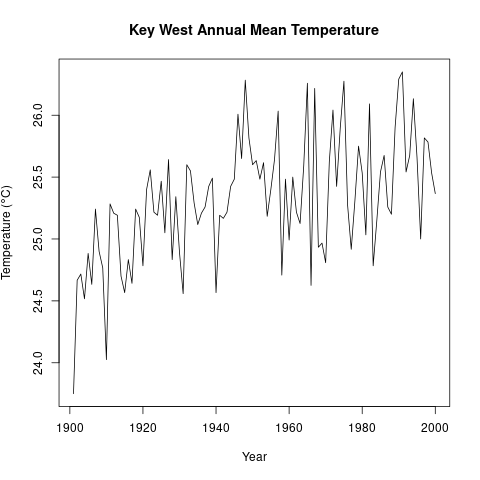
\includegraphics[width=\textwidth]{02_time.png}
    \caption{Key West annual mean temperatures throughout the 20th century}
    \label{fig:time}
\end{subfigure}
\hfill
\begin{subfigure}{0.45\textwidth}
    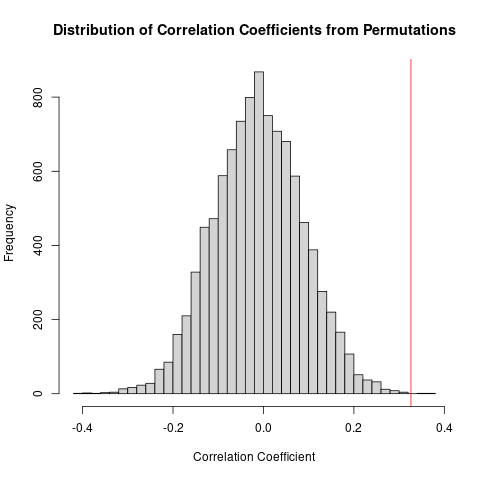
\includegraphics[width=\textwidth]{02_corr.png}
    \caption{Distribution of correlation coefficients from permutations, with the red line representing the p-value obtained from the real data.}
    \label{fig:corr}
\end{subfigure}
\end{figure}

Correlation coefficients from permutations ranged between 0.38 and -0.40, with a mean of 0 (see Fig. \ref{fig:corr}).


\end{document}

